\chapter{\uppercase{Modeling}} \label{ch:modeling}

Though the methods presented in this thesis may be useful on a variety of
control systems, the primary application described herein is to mechanical
systems.
%
In particular, this work attempts to demonstrate the application of energy
shaping in bipedal robotic locomotion.
%
Walking is characterized by phases of continuous motion with periodic discrete
impacts.
%
The combination of continuous and discrete dynamics motivates the use of hybrid
systems methods for modeling and controlling bipeds.
%
This chapter presents a development of modeling for hybrid systems which is
sufficient to understand the theory and examples present in this thesis.
%

\section{Hybrid Dynamical Systems}

Hybrid dynamical systems are systems which combine continuous and discrete
dynamics.
%
By their nature, they provide a useful framework for modeling mechanical systems
with impacts.
%
The combination of dynamics motivates the use of hybrid systems in modeling
numerous physical phenomena including bipedal walking, which is the motivating
example most pertinent to this thesis.
%

Hybrid dynamical systems have seen widespread use and comprehensive formal
development over the years;
%
see, e.g., \cite{Branicky1998, Goebel2009, Grizzle2014, Schaft2000,
  Westervelt2007}.
%
Other frameworks exist for modeling the same physical phenomena such as
differential inclusions as discussed in \cite{Filippov1988} but hybrid systems
methods are becoming increasingly popular.

With the goal of modeling a mechanical system exhibiting both continuous and
discrete dynamics, consider a hybrid dynamical system with total energy
$\E\argsqdq$ where the coordinates $\q \in \Q$ take values in the {\em
  configuration space} $\Q$ and the velocities are in the tangent bundle,
$T\Q$.
%
For ease of exposition, let the generalized coordinates of the system be
represented by $\argsqdq = \x \in \X$ where $\X$ is the state space.
%
The evolution of the system depends on a {\em unilateral constraint}, $h :
\Q \to \Rnn$, which can be used to define the {\em guard} or {\em switching
  surface}.
%
In the case of a bipedal robot with simple foot behavior, a common selection for
the unilateral constraint is the height of the swing foot, i.e., $\h\arx =
\hnsf\argsq$.
%
Through definition of an appropriate unilateral constraint on a hybrid system
whose zero crossings correspond to discrete transitions certain properties of
the system follow.
Defining a unilateral constraint to be non-negative leads a definition of the
{\em domain of admissibility} as
%
\begin{align}
  \label{eq:domain}
  \D = \left\{ \x \in T\Q : \h\arx \geq 0 \right\},
\end{align}
%
which describes the admissible states of the system.
%
The boundary at the zero level set of $\h\arx$ naturally gives rise to the
switching surface,
%
\begin{align}
  \label{eq:guard}
  \Guard &= \left\{ \x \in \D \subset T\Q : \h\arx = 0 \mbox{ and } \doth\arx <
    0 \right\}.
\end{align}
%
Using these spaces, an uncontrolled hybrid system can be expressed as
%
\begin{align}
  \HS = \left\{
  \begin{array}{l l}
    \dx = \xf(\x), & \xm \in \D \setminus \Guard,\\
    \xp = \Delta(\xm), & \xm \in \Guard,
  \end{array}\right.
  \label{eq:hsys}
\end{align}
%
where $\xf\arx$ and $\xg\arx$ are smooth vector fields and $\Delta : \Guard \to \D
\setminus \Guard$ is a smooth map called the reset map (see, e.g.,
\cite{Morris2005}).
%
In addition, $\xm\argt = \lim_{\tau \nearrow t} \x\argtau$ and $\xp\argt =
\lim_{\tau \searrow t} \x\argtau$ are the left and right limits of the solution
$\x\argt$, respectively.
%
For compactness of notation, a hybrid system is sometimes written as
\begin{align*}
  \HS = (\D, \, \Guard, \, \Delta, \, \xf).
\end{align*}
as in \cite{Sinnet2009}.
%
Under the action of control effort $\uu$, the corresponding hybrid control
system has the form
%
\begin{align}
  \HCS = \left\{
  \begin{array}{l l}
    \dx = \xf\arx + \xg\arx \, \uu, & \xm \in \D \setminus \Guard,\\
    \xp = \Delta(\xm), & \xm \in \Guard,
  \end{array}\right.
  \label{eq:hcsys}
\end{align}
%
for control values in a set of {\em admissible controls}, $\U \subseteq \R^{m}$.
%
As with hybrid systems, hybrid control systems are sometimes written more
compactly:
\begin{align*}
  \HCS = (\D, \, \Guard, \, \U, \, \Delta, \, \xf, \, \xg).
\end{align*}

Using these basic formalisms of hybrid systems, the next three sections describe
how to construct hybrid system formulations for mechanical systems.

\section{Solutions to Hybrid Systems} \label{sec:hsys-sol}
Consider the hybrid system $\HS$ given in \eqref{eq:hsys}.
%
The solution involves the differential equation
\begin{align}
  \label{eq:xdot}
  \dx = \xf\arx
\end{align}
which defines the continuous dynamics of \eqref{eq:hsys} as well as the reset
map
\begin{align}
  \label{eq:rmap}
  \dxp = \Delta\arxm
\end{align}
which defines the discrete dynamics.
%
Solutions to the differential equation governing the dynamics are valid on an
open subset of $\R^{n}$, namely the domain, $\D \subset \R^{n}$.
%
The vector field is assumed to be continuously differentiable viz. $\xf \in
C^{1}(\D)$.
%
For an initial condition $\x_{0} \in \D$, the solution $\x\argt$ will evolve
according to \eqref{eq:xdot} until it reaches the edge of $\D$, intersecting
the guard $\Guard$ by assumption (transversality).

Define the {\em flow} of the differential equation as
\begin{align*}
  \flowt(t_{0}, \x_{0}) = \x_{0} + \int_{t_{0}}^{t} \! \xf(\x\argtau) \ d\tau.
\end{align*}
%
This function represents a trajectory of the differential equation
\eqref{eq:xdot} which starts at time $t_{0}$ with initial value $\x_{0}$ and
flows until time $t$ with final state $\arx\argt$.
%
From this expression, it is clear also that there is a {\em time-to-impact} function
$\TI : \D \to \Rnn$ guaranteed by the implicit function theorem as follows:
%
using the unilateral constraint $\h$ associated with the hybrid system, define
the function
\begin{align*}
  N(t, \x) = \h(\flowt\arx).
\end{align*}
%
This function is continuous in $\x$.
%
By the implicit function theorem and the assumption of
transversality---specifically, valid solutions do not travel along the guard
viz. $\doth\arx \ne 0$---there exists a unique function $\TI(\x)$ defined and
continuous for any given point in $\D$.
%
This function maps a given state $\x$ to the time until that solution crosses
the guard.
%

Stability analysis of hybrid systems often involves a method attributable to
\Poincare{}.
%
This method is widely used in various types of systems including continuous
systems, discrete systems, and hybrid systems; for some examples, see
\cite{Guckenheimer1983, Parker1989, Perko2001, Grizzle2014}.
%
The method of \Poincare{} sections allows one to select a \Poincare{} section
at which the system is sampled.
%
The \Poincare{} section can be chosen such that a discrete system is created by
sampling with either a time-based or event-based rule.
%
For mechanical systems with impacts, an event-based rule is constructed by
choosing the \Poincare{} section to correspond to impact events.
%
More specifics about the \Poincare{} are introduced in
\chapref{ch:energy-shaping}.

Using the time-to-impact function, one can define the {\em \Poincare{} first
  return} map, $\P : \Guard \to \Guard$, as the following partial map:
%
\begin{align}
  \label{eq:poincare-map}
  \P\arx  = \Delta(\flow_{\TI\arx}\arx), \ \forall \x \in \Guard.
\end{align}
%
One can see that the \Poincare{} map is also continuous.
%
Stability of the hybrid system can then be analyzed by examining stability of
the discrete system \cite{Morris2009} defined by the \Poincare{} map
\eqref{eq:poincare-map}.
%
A solution $\flowt(t_{0}, \x_{0})$ is {\em periodic} if there exists a $T > 0$
such that
\begin{align*}
  \x\argzero = \flow_{T}(\x(0)),
\end{align*}
%
A set $\Orbit \subset \D$ is a {\em periodic orbit} if
\begin{align*}
  \Orbit = \{ \Delta(\flowt(\x)) : 0 < t < \TI(\x\argzero) \}
\end{align*}
for some periodic solution $\flowt(t_{0}, \x_{0})$.

For hybrid systems, a discrete event may occur periodically throughout the flow
leading to discontinuities.
%
The periodic orbit in such a case is not closed.
%
Beginning at time $t_{0}$, a solution to \eqref{eq:hsys} evolves according to
\eqref{eq:xdot} until the trajectory reaches the hypersurface $\Guard$ at time
$t_{1}$.
%
At this point, the reset map instantaneously alters the state according to
\eqref{eq:rmap} which causes a discontinuity in the solution $\x\argt$ resulting
in a discrete state update law which yields a new initial condition, $\xp(t_{1})
= \Delta(\xm(t_{1})).$
%
From this new initial condition, the solution then continues to evolve from
\eqref{eq:xdot}.

Because the discrete dynamics is considered to operate on the solution
instantaneously, it is important to distinguish between the pre-impact state,
\begin{align*}
  \x(t^{-}) = \xm = \lim_{\tau \nearrow t} \x\argtau,
\end{align*}
which occurs at time $t^{-}$, and the post-impact state,
\begin{align*}
  \x(t^{+}) = \xp = \lim_{\tau \searrow t} \x\argtau,
\end{align*}
which occurs at time $t^{+}$.
%
The discrepancy in left- and right-hand limits is due to the discontinuity in
solutions introduced by the reset map.
%

A solution can be created by piecing together these solutions which each
describes the evolution of coordinates as the state flows from a point on
$\Guard$ through the domain $\D$ until it intersects $\Guard$ again.
%
Such solutions are often called {\em hybrid flows} or {\em hybrid executions}.
%
Formally, a hybrid flow of \eqref{eq:hsys} is a tuple
\begin{align*}
  \Upsilon^{\HS} = \left( \cK, \cI, \cC \right)
\end{align*}
where $\cK = \{0, 1, 2, \ldots\} \subseteq \N$ is a finite or countably
infinite {\em indexing set}, $\cI = \left\{I_{k}\right\}_{k \in \cK}$ is a {\em
  hybrid interval} with $I_{k} = \left[t_{k}, t_{k+1}\right]$, and $\cC =
\left\{c_{k}\right\}_{k \in \cK}$ is a collection of continuous solutions of
$\xf\arx$, i.e., ${\dot c}_{k}\argt = \xf(c_{k}\argt) \, \forall k \in \cK$.
%
In order to maintain consistency, the following conditions must be met:
%
\begin{enumerate}
\item $c_{k}(t_{k+1}) \in \Guard$
\item $\Delta(c_{k}(t_{k+1})) = c_{k+1}(t_{i+1})$
\end{enumerate}

Further details about solutions of hybrid systems also appears in
\chapref{ch:energy-shaping}.
%
For additional notions of solutions in hybrid systems, see \cite{Filippov1988,
  Goebel2009, Haddad2001, Lygeros2003, Ye1998}.

\section{Stability Definitions} \label{sec:hsys-stability}

Because of the unique nature of hybrid systems, analysis of stability requires
special treatment which is distinct from continuous-time systems and more
closely parallels that used for discrete-time systems.
%
In order to understand the theory presented in this work, it is necessary to
understand not only the stability of hybrid systems but also the stability of
continuous systems and discrete systems which partly comprise hybrid systems.
%
This section presents formal definitions of stability (based on
those found in \cite[Ch. 4]{Khalil2002}) which are key to understanding the
results presented in this work.
%
For more on stability, see, e.g., \cite{Khalil2002, Teschl2012,
  Vidyasagar1993}.
%
For comments on the literature, see \secref{sec:literature-stability}.

\subsection{Continuous Systems}
This work is chiefly concerned with autonomous systems of the form
\begin{align}
  \label{eq:autsys}
  \dx = \xf\arx
\end{align}
where $\xf : \D \to \Rn$ is a locally Lipschitz vector field valid on some
domain $\D \subset \Rn$.
%
Without loss of generality, suppose that the system \eqref{eq:autsys} has an
equilibrium point at the origin;
%
in other words, $\xf\argbzero = \boldzero$.
%
\begin{definition}
  The equilibrium point $\x = \boldzero$ is stable if, for each $\epsilon > 0$,
  $\exists \ \delta > 0$ such that
  \begin{align*}
    \nxzero < \delta \Rightarrow \nxt < \epsilon \ \forall \ t
    \geq 0.
  \end{align*}
  The equilibrium point is unstable if it is not stable.
\end{definition}

In addition to the above definition, a stricter forms of stability is defined as
follows:
%
\begin{definition}
  The equilibrium point $\x = \boldzero$ is {\bf asymptotically stable} if it is
  stable and $\delta$ can be chosen such that
  \begin{align*}
    \nxzero < \delta \Rightarrow \lim_{t \to \infty} \x\argt = \boldzero.
  \end{align*}
\end{definition}

Further, an even stronger form of stability is of interest in this work:
%
\begin{definition}
  The equilibrium point $\x = \boldzero$ is {\bf exponentially stable} if there
  exist real constants $c, k, \lambda > 0$ such that
  \begin{align*}
    \nxt \leq k \nxtnaught e^{-\lambda (t - t_{0})} \ \forall \ \nxtnaught < c.
  \end{align*}
\end{definition}


\subsection{Discrete Systems}

In analogy to continuous systems, consider the autonomous system which satisfies
the difference equation
\begin{align}
  \label{eq:disc-sys}
  \x_{k+1} = f(\x_{k}).
\end{align}
where $f : \D \to \D$ is a locally Lipschitz vector field valid on some domain
$\D \subset \Rn$.
%
Without loss of generality, suppose that the system \eqref{eq:disc-sys} has an
equilibrium point at the origin;
%
in other words, $f\argbzero = \boldzero$.
%
\begin{definition}
  The equilibrium point $\x = \boldzero$ of \eqref{eq:disc-sys} is stable if,
  for each $\epsilon > 0$, $\exists \delta > 0$ such that
  \begin{align*}
    \nxkzero < \delta \Rightarrow \nxk < \epsilon \ \forall \ k
    \geq 0.
  \end{align*}
  The equilibrium point is unstable if it is not stable.
\end{definition}
%
Similar to continuous systems, asymptotic stability is defined as follows:
%
\begin{definition}
  The equilibrium point $\x = \boldzero$ of \eqref{eq:disc-sys} is {\bf
    asymptotically stable} if it is stable and $\delta$ can be chosen such that
  \begin{align*}
    \nxkzero < \delta \Rightarrow \lim_{k \to \infty} \xk = \boldzero.
  \end{align*}
\end{definition}
%
Exponential stability for discrete systems is formally defined as follows:
%
\begin{definition}
  The equilibrium point $\x = \boldzero$ of \eqref{eq:disc-sys} is {\bf
    exponentially stable} if there exist real constants $\alpha, \beta, c> 0$
  such that, for all $\nxknaught < c$ and $k \geq k_{0}$,
  \begin{align*}
    \nxk \leq \beta \nxknaught^{\alpha}.
  \end{align*}
\end{definition}
%
These definitions will tie into the work later in \chapref{ch:energy-shaping}.


\section{Rigid Body Kinematics}

At its core, the modeling of complex mechanical systems involves a
straightforward, if often complicated, application of Newton's Second Law (see
\cite{Feynman1964}), namely,
\begin{align*}
  F = m \, a,
\end{align*}
which expresses the basic property of physics that applying a force to a massive
object induces a particular acceleration.
%
Through the property of superposition, this relationship eventually leads to the
standard dynamic model of a robot given later in \eqref{eq:eom}.
%
But despite the development of complex models, all physics-based models
fundamentally demonstrate Newton's Second Law.

Consider a three-dimensional rigid body with no contact assumptions; i.e., the
body is free to move in space.
%
With the dynamics of the system being dominated by Newton's laws of motion
\cite{Feynman1964}, the state of the system can be expressed by associating a
reference frame to a fix pointed on the body and using coordinates which express
the position and orientation of this point with respect to a global frame or the
world frame.
%
In three-dimensional space, this transformation between world frame and robot
frame can be parameterized with six coordinates: three representing the
Euclidean position and three respresenting, for example, an Euler angle--based
derivation, namely, the product of three rotation matrices
\cite[Ch. 7]{Baruh1998}.
%
The set of all admissible configurations for such a body represents a specific
topological space referred to as the {\em special Euclidean group}, $\SE(3)$.
%
This group can be thought of as the Cartesian product of the position and
orientation of a body, i.e., $\SE(3) = \R^3 \times \SO(3)$, where $\SO(3)$ is
the {\em special orthogonal group} which can be understood as
\begin{align*}
  \SO(n) = \left\{ R \in \R^{n \times n} : R R^T = I, \det R = 1 \right\}.
\end{align*}
For more information on these topological spaces, consult
\cite[Ch. 2]{Murray1994}.


Newton's laws eventually lead to the understanding that the motion of such a
system can be captured by the following dynamic model:
\begin{align*}
  I_{x} \dot{\omega}_{x} + (I_{z} - I_{y}) \omega_{y} \omega_{z} &= M_{x}\\
  I_{y} \dot{\omega}_{y} + (I_{x} - I_{z}) \omega_{z} \omega_{x} &= M_{y}\\
  I_{z} \dot{\omega}_{z} + (I_{y} - I_{x}) \omega_{x} \omega_{y} &= M_{z}\\
  m \dot{v}_{x} &= F_{x},\\
  m \dot{v}_{y} &= F_{y},\\
  m \dot{v}_{z} &= F_{z},
\end{align*}
where linear and angular velocity are represented by $v$ and $\omega$,
respectively, and the corresponding accelerations are shown as time
derivatives.
%
The applied forces and moments are shown as $F$ and $M$, respectively, and the
$I_{x}$, $I_{y}$, and $I_{z}$ terms are the principal moments of inertia about
the appropriate axes.
%
As one might guess, this requires that the fixed frame be located at the center
of mass and oriented along the principal axes of inertia; it is straightforward
to redefine the base coordinates but this form---the simplest form ---is given
for clarity of presentation.
%
For the full development of the above, see, for example,
\cite[Ch. 8]{Baruh1998}.

%\section{Kinematic Chains}

Typical robots consist of kinematic chains of rigid bodies attached with
prismatic or revolute joints, and for simplicity, the resulting dynamics
generally has the appropriate contact assumptions baked in to simplify
computation (as in \eqref{eq:eom}), but it is possible to consider
each rigid body separately and solve for the appropriate reaction forces which
can be applied through $F$ and $M$ to maintain the proper contact (this is
typically called the Newton--Euler method \cite{Hollerbach1980}).
%
For robotic motion, non-holonomic constraints act to reduce the allowable motion
and, as a consequence, there exists a minimal set of coordinates which can be
used to describe a robot's dynamics.
%
This minimal set is referred to as the {\em generalized coordinates}.


\section{Langrangian Formulation}

%\section{Spatial Vector Algebra}
%While a Lagrangian-based approach to modeling is useful for theoretical
%applications and smaller systems, its shortcomings quickly emerge as systems
%grow in complexity.
%
%Perhaps more than anything else, this poor scalability stems from the need to
%successively multiply rotation matrices in symbolic form resulting in
%progressively larger expressions.
%
%Moreover, as complexity grows, it becomes is increasingly difficult to glean
%any useful bit of intuition from examining the expressions in symbolic form.

With the basic understanding provided in the previous section, some additional
details will now be provided.
%
Begin with a bipedal robot in either two or three dimensions---the discussions
herein are applicable to either case.
%
Then construct a Lagrangian for the biped in a general position---specifically,
no assumptions are made on ground contact---and use non-holonomic constraints to
enforce ground contact conditions.

Let $R_{0}$ be a fixed inertial or world frame and let $\Rb$ be a reference
frame attached to the body of the biped with position $p_{b} \in \R^{3}$ and
orientation $\phi_{b} \in \SO(3)$ where $\SO(n)$ represents the special
orthogonal group in $n$ dimensions (see \cite{Conway1985}).
%
Let $\qs \in \Qs$ represent a choice of {\em body} or {\em shape
  coordinates} for the robot with $\Qs$ the configuration space.
%
Herein, $\qs$ represents the relative angles between adjacent links of the
robot as shown later in \figref{fig:shapecoords}.
%
The {\em generalized coordinates} are then found by combining the shape
coordinates with the position and orientation of the body-fixed frame, $\Rb$,
viz.
%
\begin{align*}
  \q = (p_{b}, \phi_{b}, \qs) \in \Q = \R^{3} \times \SO(3)
  \times \Qs,
\end{align*}
%
where $\Q$ is the generalized configuration space.

The Lagrangian of a bipedal robot, $\Lag : T\Q \to \R$, can be stated in terms
of the kinetic energy, $K : T\Q \to \R$, and the potential energy, $U : \Q \to
\R$, as:
%
\begin{align*}
  \Lag\argsqdq = K\argsqdq - U\argsq.
\end{align*}
%
For robots, the kinetic energy has the form
\begin{align*}
  K\argsqdq = \dq^{T} \M\argsq \, \dq.
\end{align*}
where $\M\argsq$ is a manipulator inertia matrix which has the property of
being symmetric and positive definite.
%
The Euler--Lagrange equation can be used to find the equations of motion, which,
for robotic systems \cite[pp.~171]{Murray1994}, are written:
%
\begin{align}
  \label{eq:eom}
  \M\argsq \, \ddq + \HCor\argsqdq = \B\argsq \, \uu
\end{align}
%
where, here, $\M\argsq$, the manipulator inertia matrix, and $\B\argsq$, the
torque distribution matrix, only depend on $\q$, $\uu$ is a vector of applied
torques, and
\begin{align*}
  \HCor\argsqdq = \CCor\argsqdq \, \dq + \G\argsq
\end{align*}
contains terms resulting from the Coriolis effect, centrifugal forces, and
gravity grouped into a single vector.
%
The contribution from gravity is related to the potential energy:
\begin{align*}
  \G\argsq = \pd{U\argsq}{\q}.
\end{align*}
%
The elements of $\CCor\argsqdq$ can be found by computing the Christoffel
symbols of $\M\argsq$:
\begin{align*}
  \CCor_{ij}\argsqdq = \frac{1}{2} \sum_{k = 1}^{n} \left( \pd{\M_{ij}}{\q_{k}} +
    \pd{\M_{ik}}{\q_{j}} - \pd{\M_{kj}}{\q_{i}} \right) \dq_{k}.
\end{align*}
%
See \cite[pp.~170]{Murray1994} for more information.

Equation \eqref{eq:eom} is the simplest dynamic model of robotic motion and does
not include any contact constraints.
% 
This is not necessary a problem if one reduces the coordinates $\q$ by locating
the body-fixed reference frame $\Rb$ at a stationary point fixing certain
degrees of freedom, thereby factoring in ground contact constraints.
%
To understand this, consider the following example:

\begin{figure}[t!]
  \centering
  \def\svgwidth{.5\columnwidth}
  \input{figs/cg2d_reduced_coordinates.eps_latex}
  \caption[Example robot coordinates for a compass-gait biped.]{Example robot
    coordinates for a compass-gait biped.
    % 
    The body-fixed frame $\Rb$ is located at the interface between the stance
    foot and the ground.
    %
    The coordinate $\phi_{b}^{y}$ tracks the orientation of $\Rb$ relative to
    a fixed world frame.
    %
    The only body or shape coordinate for this simple model is $\q_{1}$.}
    \label{fig:compass_gait_reduced_coordinates}
\end{figure}

\begin{exmp}
  \label{ex:compass_gait_reduced_coordinates}
  The dynamics of a 2D model with point feet that walks in the
  $x$--$z$ plane along the $x$-axis as that shown in
  \figref{fig:compass_gait_reduced_coordinates} can be modeled with the
  coordinates $q = (\phi_{b}^{y}, \q_{1})$ using \eqref{eq:eom}.
\end{exmp}


\section{Constraining Forces}

As mentioned, the motion of a rigid-body robot is governed by \eqref{eq:eom}.
%
The formulation of the equation, however, does not allow for analysis of
reaction forces.
%
This models takes into account reaction forces but they do not appear in the
equations as they must be included in the form of kinematic constraints which
alter the form of the dynamics by fixing coordinates as in \exmpref{ex:compass_gait_reduced_coordinates}.

In some cases, one may wish, for a variety of reasons, to compute the reaction
forces themselves.
%
For those who study materials and mechanism design of bipedal robots, it may be
important to understand the forces present at the joints or at the feet to aid
in design.
%
Control theorists may wish to understand the moment at the stance foot in order
to design gaits in which the foot does not rotate inadvertently.
%
In addition, researchers may wish to study foot-strike which requires the use of
impulsive constraining forces.
%
For these reasons and others, it is important to consider a more generalized
model that, at the very least, includes reaction forces at the feet.

This section will show how constraints can be added to the standard robotic
model.
%
There are two different types of constraints which should be distinguished; see
\cite[Ch. 6]{Murray1994} for further details.
%
Holonomic constraints act to restrict the motion of a system to a smooth
hypersurface of the configuration space $\Q$.
%
Similarly, non-holonomic constraints act to restrict the motion of a system
through a restriction on velocity.
%
The modeling of constraints necessary for robots can generally be handled by
considering only non-holonomic constraints, which have the form
\begin{align}
  \label{eq:holocon}
  \J\argsq \, \dq = \mathit{constant},
\end{align}
where $\J\argsq$ can be thought of as a Jacobian matrix.
%
It is assumed that the constraints are linearly independent and thus $\J\argsq$
has full row rank.
%
Intuitively, the rows of $\J\argsq$ represent maps to velocities of the
system---i.e., for $\J_{i}\argsq$ which is the $i^{\mathrm{th}}$ row of
$\J\argsq$, the quantity $\J_{i}\argsq \, \dq$ represents an output
velocity---which are to be restricted to a constant.
%
Generally and all throughout this thesis, the constant is zero; that is, the
constraints are designed to prevent any motion rather than enforce constant,
non-zero velocity.

Revisiting the standard robot model, consider augmenting the model to allow
additional forces for imposing non-holonomic constraints:
%
\begin{align}
  \label{eq:eom-lambda}
  \M\argsq \, \ddq + \HCor\argsqdq + \J^{T}\argsq \, \lambda = \B\argsq \, \uu.
\end{align}
%
In the literature, $\lambda$ is often referred to as a Lagrange multiplier
\cite[\S 4.10]{Baruh1998} and $\J^{T}\argsq$ is a map from the space in which
the output velocity constraints are represented (output space) to joint space
and thus the constraining forces in joint space are given by
%
\begin{align*}
  F_{\mathit{c}} = \J^{T}\argsq \lambda.
\end{align*}
The idea is to solve \eqref{eq:eom-lambda} for $\lambda$ in terms of $\q$,
$\dq$, and $u$ such that \eqref{eq:holocon} is satisfied.
%
Differentiating \eqref{eq:holocon} results in
\begin{align*}
 \dJ\argsqdq \, \dq + \J\argsqdq \, \ddq = 0.
\end{align*}
%
Then solving \eqref{eq:eom-lambda} for $\ddq$ and substituting into the above
results in
\begin{align*}
  \dJ\argsqdq \, \dq + \J\argsqdq \, \M^{-1}\argsq \left(\B\argsq \, \uu
    -\HCor\argsqdq - \J^{T}\argsq \, \lambda \right) = 0.
\end{align*}
Finally, solving for $\lambda$ gives
\begin{align*}
   \lambda = \left( \J\argsqdq \, \M^{-1}\argsq \, \J^{T}\argsq \right)^{-1}
   \left( \dJ\argsqdq \dq + \J\argsqdq \, \M^{-1}\argsq \left(\B\argsq \, \uu
    -\HCor\argsqdq\right) \right).
\end{align*}
%
This formulation can be used to treat robots in a generalized configuration
with non-holonomic constraints such as ground contact.

Using the developments in this section, the next section will show how to treat
impacts which require constraining forces.

\section{Discrete Impacts}

When studying bipedal walking, it is important for the sake of thoroughness, to
consider impacts and their effect on the motion of a system.
%
Simple models like the linear inverted pendulum model ignore foot strike which
results in a greater gap between simulation and experiment.
%
For more on the different models and how impacts are treated, see
\secref{sec:literature-bipeds}.
%
Non-smooth mechanics is a complicated topic; more detail can be found in, for
example, \cite{Brogliato1996, Kozlov1991}.
%
The mechanics of non-smooth impacts has been addressed for tool use in
\cite{Gorinevsky1997, Siciliano1999}.
%
In addition to the rigid models considered in this thesis (as those treated by
Hurmuzlu and Marghitu \cite{Hurmuzlu1994}), elastic impacts and model
deformation have also been considered \cite{Chapnik1991, Wei1993}.

For the purposes of this work, an impact is considered to occur when a rigid
body (the foot) comes into contact with the ground.
%
For simplicity, impacts are assumed to be rigid and plastic.
%
Consider the extended robot dynamics equation \eqref{eq:eom-lambda}.
%
The Lagrange multiplier $\lambda$ can be used with impacts by considering it to
be representative of impulsive forcing.
%
Denote by $\dqm = \lim_{\tau \nearrow t} \dq\argtau$ and $\dqp = \lim_{\tau
  \searrow t} \dq\argtau$ the left and right limits to the solution
$\dqe\argt$, respectively.
%
Thus $\dqm$ and $\dqp$ respectively represent pre- and post-impact velocities.
%
In addition, by assumption the configuration coordinates are continuous in time
so $\qm = \qp = \q$.
%
Assuming actuators do not produce impulsive forces and integrating the model
\eqref{eq:eom-lambda} results in
\begin{align}
  \label{eq:impulse}
  \M\argsq(\dqp - \dqm) = \J^{T}\argsq \lambda\argsqdqm
\end{align}
where
\begin{align*}
  \int_{t^{-}}^{t^{+}} \! \lambda\argsqdqtau \, d\tau.
\end{align*}
%
Based on the desired constraints, one can construct a Jacobian matrix,
$J\argsq$, whose rows contain individual constraints.
%
Combining \eqref{eq:eom-lambda} with \eqref{eq:impulse} results in the impact model:
\begin{align*}
  \left(\begin{array}{c c}
      \M\argsq & -\J^{T}\argsq\\
      \J\argsq & \boldzero
    \end{array}\right)
  \left(\begin{array}{c}
      \dqp\\
      \lambda\argsqdqp
    \end{array}\right) =
  \left(\begin{array}{c}
      \M\argsq \, \dqm\\
      \boldzero
    \end{array}\right)
\end{align*}
%
This model is used throughout this thesis wherever impacts arise.

The information provided thus far is sufficient to handle simple bipeds with
point feet but for more complex models, the definitions for hybrid systems must
be expanded.
%
This will be done in the next section.



\section{Complex Domain Structure} \label{sec:complex-models}

%Bipedal robotic walking exhibits both discrete and continuous behavior; it is,
%therefore, natural to model bipedal robots as hybrid systems.
%
A large portion of the research on bipedal robotic walking focuses on models of
robots with point feet or flat-foot walking.
%
This results in a simple hybrid model with a single domain which can be treated
using the methods described earlier in this chapter.
%
This idealization results in walking gaits which lack some of the distinguishing
characteristics of human locomotion.
%
In particular, the foot behavior of human walking is highly recognizable and
sets human walking apart from the flat-footed gaits seen on many of the early
bipedal robots.

Under a more general view, a human walking gait can be seen to consist of
multiple {\em phases} or {\em domains}---in each domain, the system evolves in a
continuous fashion according to a dynamic model derived from a Lagrangian
modeling the mechanical system on that domain.
%
The dynamic model will vary depending on which points on the robot are in
contact with the ground---having points in contact with the ground introduces
kinematic constraints on the system.
%
At a certain point in each domain, i.e., when the contact points change, the
model will discretely change to another phase of walking with a different
dynamic model and different control.
%
In the case of an end-effector on the robot coming into contact with the
environment, impulsive forces act on the contact point which instantaneously
alter the velocity of the system.
%
%This combination of continuous and discrete phenomena is the fundamental
%concept underlying hybrid systems.

In this section, a formalism for multi-domain hybrid systems is introduced and a
discussion of how the equations of motion of a robot together with a temporal
ordering of discrete events, i.e., change in contact points, completely
determine the hybrid model of a system.
%
More specifically, to model bipedal robots, one need only consider the domain
breakdown and the Lagrangian on each domain.
%
Details are provided to show how the breakdown can be derived by considering the
kinematic constraints imposed on the system throughout the course of a step.


\subsection{Formal Definitions}
%{\em Hybrid systems} or {\em systems with impulse effects}\cite{GAP01}\xspace have been studied extensively in a wide variety of contexts and have been used to model a wide range of bipedal robotic systems.\cite{GCAS10}\xspace This section introduces a definition of hybrid systems applicable to bipedal walking.

Steady state bipedal walking is naturally periodic with discrete impacts leading
to different walking phases.
%
Therefore, when studying walking, one should consider multi-domain hybrid
systems with a temporal ordering of events, i.e., systems in which the domain
graph is a {\em directed cycle}:

\begin{figure}[t]
  \centering
  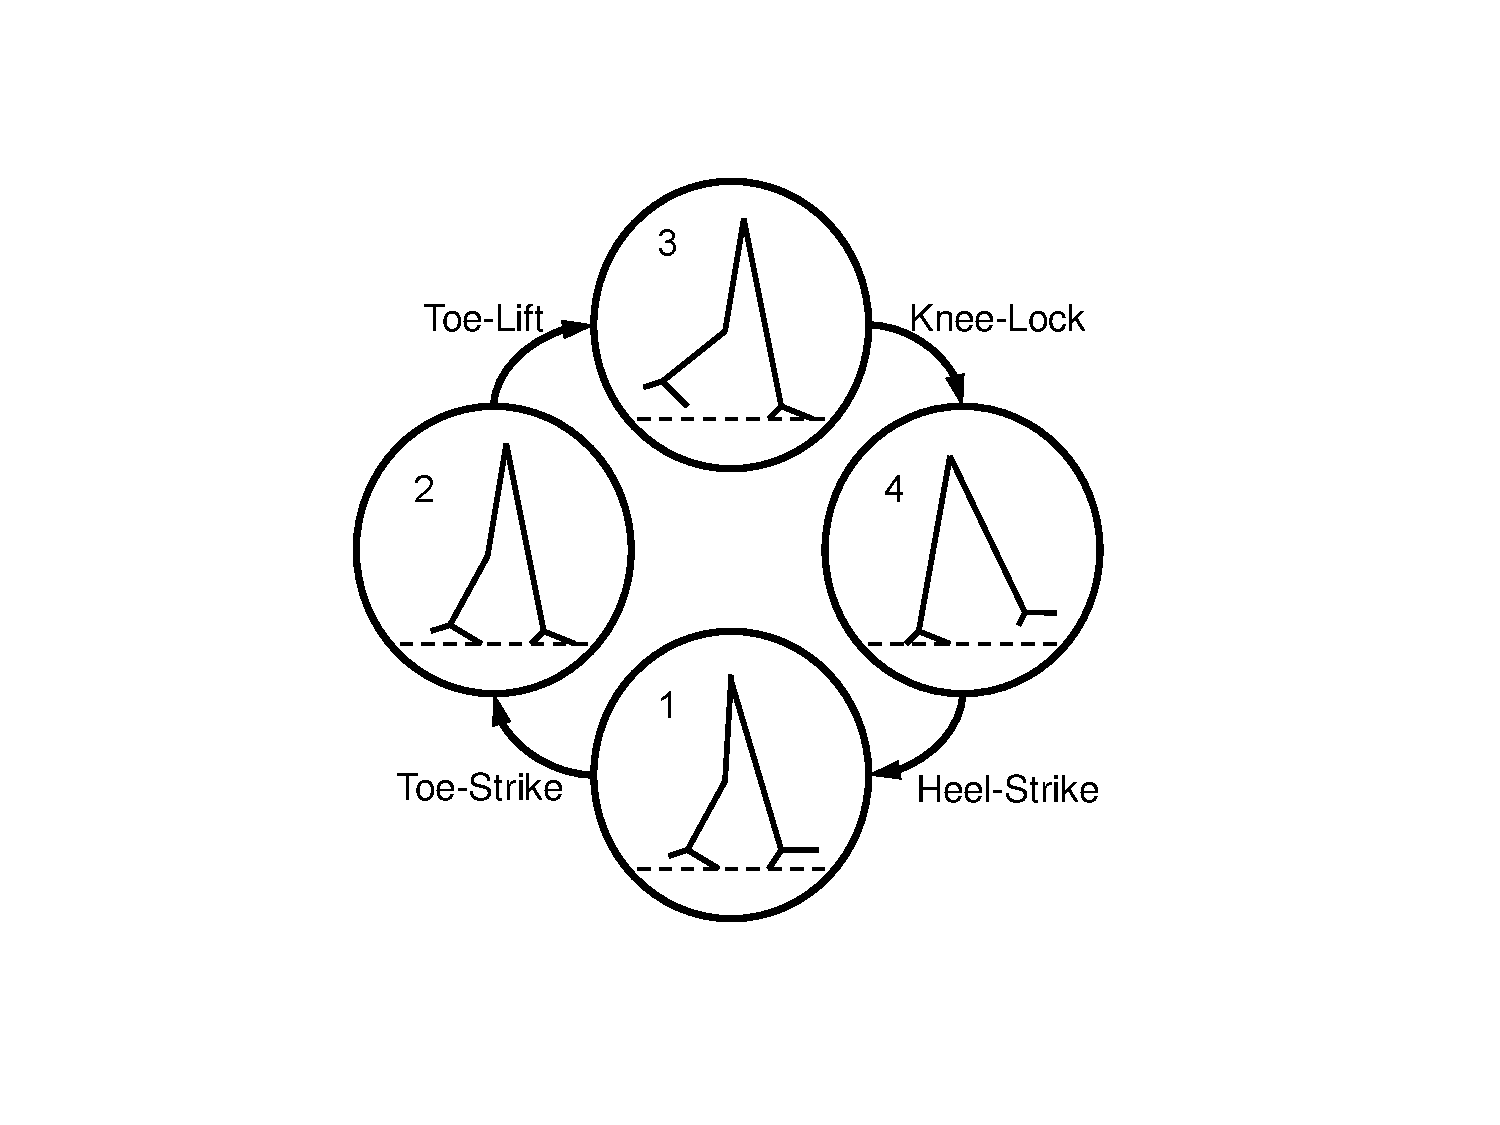
\includegraphics[width=0.8\columnwidth]{domaingraph}
  \caption[An example of a {\em domain breakdown}.]{An example of a {\em domain
      breakdown}.
    %
    That is, a combination of discrete phases of a walking gait with a specific
    temporal ordering. The red dots indicate which constraints are enforced in
    each discrete phase (or domain).
    %
    The domain labels are selected based on which event causes a given domain to
    transition to the next.}
  \label{fig:domaingraph}
\end{figure}

\begin{definition}
  A {\bf directed cycle} is a graph $\Gamma = (V, E)$, with $V$ a set of {\bf
    vertices} and $E$ a set of {\bf edges}---for an edge $\einE$, denote the
  {\bf source} by $\sor(e)$ and the {\bf target} by $\tar(e)$---in which the
  vertices and edges can be written
  %
  \begin{align}
    \nonumber
    V &= \left\{\vo_{1}, \, \vo_{2}, \, \ldots, \, \vo_{p}\right\},\\
    \label{eq:directedcyclep}
    E &= \left\{e_{1} = \{\vo_{1}, \vo_{2}\}, \, e_{2} = \{\vo_{2}, \vo_{3}\}, \,
      \ldots, \, e_{p} = \{\vo_{p}, \vo_{1}\}\right\},
  \end{align}
  %
  where $p$ is the number of discrete domains in the corresponding hybrid
  model.
\end{definition}

This concept is illustrated in the following example, which will be used later
in \chapref{ch:hic}:

\begin{exmp} \label{universalgraph}
  The domain breakdown pictured in \figref{fig:domaingraph} has an underlying
  graph that is a directed cycle;
  %
  the graph is given by $\Gamma = (V, \, E)$.
  %
  In particular, there are four vertices and four edges with
  %
  \begin{align*}
    V &= \left\{\DA, \, \DB, \, \DC, \, \DD\right\},\\
    E &= \left\{\{\DA, \, \DB\}, \, \{\DB, \, \DC\}, \, \{\DC, \, \DD\}, \,
      \{\DD, \, \DA\}\right\}.
  \end{align*}
\end{exmp}

The concept of a directed cycle is a fundamental component in the formulation
of multi-domain hybrid systems:\todo{notation of \cite{Guckenheimer1995}}

\begin{definition} \label{def:hcs}
  A {\bf hybrid control system in a cycle} is a tuple,
  %
  \begin{align*}
    \HCS = (\Gamma, \, \D, \, \U, \, \Guard, \, \Delta, \, \FG),
  \end{align*}
  %
  where
  \begin{itemize}
  \item $\Gamma = (V, \, E)$ is a {\bf directed cycle},
  \item $\D = \{\Dv\}_{\vinV}$ is a set of {\bf domains} with $\Dv
    \subseteq \Xv \times \Uv$ a smooth submanifold, where $\Xv$ represents the
    state space,
  \item $\U = \{\Uv\}_{\vinV}$ with $\Uv \subseteq \Rmv$ a set of
    {\bf admissible controls},
  \item $\Guard = \{\Guarde\}_{\einE}$ is a set of {\bf guards} or {\bf
      switching surfaces}, with $\Guarde \subseteq \D_{\sor(e)}$,
  \item $\Delta = \{\Deltae\}_{\einE}$ is a set of {\bf reset maps}, with
    $\Deltae : \Guarde \to \X_{\tar(e)}$ a smooth map,
  \item $\FG = \{(\xfv, \, \xgv)\}_{\vinV}$ with $(\xfv, \, \xgv)$ a {\bf control
      system} on $\Dv$, i.e., $\dx = \xfv\arx + \xgv\arx \, \uu$ $\forall$
    $\argsxuu \in \Dv$,
  \end{itemize}
  for $\vinV$ with edge $\einE$ satisfying $\vo = \sor(e)$.
  %
  This can also be described as an indexed system with impulse effects:
  \begin{align}
    \label{eq:HCSi}
    \HCSv = \left\{
      \begin{array}{l l}
        \dx = \xfv\arx + \xgv\arx \, \uu, & \argsxuum \in \Dv \setminus
        \Guarde,\\
        \xp = \Deltae(\xm), & \argsxuum \in \Guarde,
      \end{array}\right.
  \end{align}
  The set of hybrid control systems for all domains in $V$ can be written $\HCS
  = \{\HCSv\}_{\vinV}$.
\end{definition}

\begin{definition}
  A {\bf hybrid system} is a hybrid control system with $\Uv = \emptyset$
  $\forall$ $\vinV$, e.g., any relevant feedback controllers have been
  applied, making the system closed-loop:
  \begin{align*}
    \HS = (\Gamma, \, \D, \, \Guard, \, \Delta, \, \F),
  \end{align*}
  %
  where $\F = \{\xfv\}_{\vinV}$, with $\xfv$ a (possibly non-autonomous) {\bf
    dynamical system} on $\X \subseteq \Dv$, i.e., $\dx = \xfv(\x, t)$ for
  $\vinV$ with edge $\einE$ satisfying $\vo = \sor(e)$.
  %
  The other elements are the same as those defined for hybrid control systems.
  %
  This corresponds to the following system with impulse effects:
  \begin{align}
    \label{eq:HSi}
    \HSv = \left\{
      \begin{array}{l l}
        \dx = \xfv\arx & \xm \in \Dv \setminus \Guarde,\\
        \xp = \Deltae(\xm), & \xm \in \Guarde.
      \end{array}\right.
  \end{align}
  %
  The set of hybrid systems for all domains in $V$ can be written $\HS =
  \{\HSv\}_{\vinV}$.
\end{definition}

Comparing the above definitions and \eqref{eq:HCSi} and \eqref{eq:HSi}, it is
clear that the domain of admissibility and the guard are dependent on control.
%
This dependence is a result of considering the dynamic moment of the system in
formulating these particular spaces and will be clarified further in
\secref{sec:discrete-dynamics}.


\subsection{Obtaining Hybrid Systems from Constraints}

The remainder of this section is devoted to discussing how the Lagrangian for a
biped, together with a domain breakdown (which determines the constraints at
each vertex of the associated cycle), allows one to explicitly construct a
hybrid model of the system.
%
Examples can be found throughout the literature; see, for example,
\cite{Grizzle2010, Grizzle2014, Sinnet2009}.


\subsubsection{Constraints}

The continuous dynamics of a system depends on which constraints are enforced at
any given time while the discrete dynamics depends on the change in
constraints.
%
Constraints and their enforcement are dictated by the configuration of contact
points between the system and the ground.
%
Specifically, one can define a {\em contact set} $\C = \{c_{1}, \, c_{2}, \,
\ldots, \, c_{k}\}$, with each $c_{i}$ a specific type of foot/ground contact
possible in the biped.
%
Assuming that foot contact is restricted to edges parallel to the $y$-axis
(i.e., the toe edge or the heel edge)---and this is the case in 2D as in this
work---there are four contact points of interest:
\begin{align*}
  \C =  \{\csh, \, \cst, \, \cnsh, \, \cnst\},
\end{align*}
where these constraints physically represent the stance heel, stance toe,
non-stance heel, and non-stance toe, respectively.
%
The reason for choosing this set of contact points will become clear after data
analysis.

\begin{remark}
  In some of the literature, the term non-stance is referred to as swing.
  %
  This is an artifact of point-foot bipedal models which have only single
  support and instantaneous double support (at impact).
  %
  This thesis instead uses the term non-stance due to the existence of
  noninstantaneous double support phases where there are periods with no free
  swinging behavior.
  %
  In this case the naming of the stance/non-stance legs is arbitrary;
  %
  in this thesis, the stance leg is defined as the leg holding most of the
  weight of the robot.
\end{remark}

%%%% FIX
%%%% Need to fix the motivation at the end of the preceding paragraph
%%%% Cite domain breakdown submission


%%%% FIX
%%%% Need to treat the following section in a more correct manner, e.g., flat
%%%% foot vs. toe roll
Contact points introduce {\em non-holonomic constraints}, $\eta_{c}$ for $c \in
\C$, on the system; this vector must be held constant for contact to be
maintained.
%
To construct these constraints, consider a reference frame $R_{c}$ at the
contact point $c$ such that the axis of rotation about this point (either the
heel or toe) is along the $y$-axis.
%
Let $\Rnaught^{c}\argsq$ be a rotation matrix between reference frames from
$\Rnaught$ and $\Rc$.
%
Let $\pc : \Q \to \R^{3}$ represent the position of the frame and let
$\vc\argsqdq = \dpc\argsqdq$ represent the velocity.
%
The body-fixed angular velocity of the frame can then be found:
%
\begin{align}
  \label{eq:angvelmat}
  \Omega_{c}\argsqdq &= (\Rnaught^{c}\argsq)^{T} \, \pd{\Rnaught^{c}\argsq}{\q}
  \, \dq\\
  \nonumber
  &= \left[\begin{array}{c c c}
      0 & -\wcz\argsqdq & \wcy\argsqdq\\
      \wcz\argsqdq & 0 & -\wcx\argsqdq\\
      -\wcy\argsqdq & \wcx\argsqdq & 0
    \end{array}\right].
\end{align}
%
The angular velocity vector
\begin{align*}
  \wc\argsqdq = (\wcx\argsqdq, \, \wcy\argsqdq, \, \wcz\argsqdq)
\end{align*}
is dual to the skew-symmetric matrix $\Omega\argsqdq$.
%
Furthermore,
\begin{align}
  \label{eq:linearvel}
  \vc\argsqdq = \pd{\pc\argsq}{\q} \, \dq
\end{align}
with $\pc\argsq$ the Cartesian position of the contact point $c$.
%
It is apparent from \eqref{eq:angvelmat} and \eqref{eq:linearvel} that
$\vc\argsqdq$ and $\wc\argsqdq$ are linearly dependent on $\dq$.
%
Thus, the non-holonomic constraint can be written
\begin{align*}
  \eta_{c}\argsqdq = \left[\begin{array}{c}
      \vc\argsqdq\\
      \wcx\argsqdq\\
      \wcz\argsqdq
    \end{array}\right] =
  J_{c}\argsq \, \dq.
\end{align*}
%
Therefore, it is possible to find the associated Jacobian matrix through
differentiation:
%
\begin{align*}
  \Jc\argsq = \pd{\eta_{c}\argsqdq}{\dq}.
\end{align*}
%
In the case of a 2D biped, the treatment is exactly the same but
\begin{align*}
  \eta_{c}\argsqdq = (\vcx\argsqdq, \, \vcz\argsqdq).
\end{align*}
%
The end result of this choice of coordinates is a non-holonomic constraint which
enforces the condition $\eta_{c}\argsqdq = \mathrm{constant}$---this fixes the
contact point to the ground but allows rotation about the heel or toe depending
on the specific type of contact.
%
It is useful to express the collection of all non-holonomic constraints in a
single matrix $\eta\argsqdq \in \R^{20 \times 4}$ as:
\begin{align*}
  \eta\argsqdq \!\! = \!\!\! \left[\!\!\begin{array}{c c c c}
    \! \eta_{\sth}\argsqdq \! & 0 & 0 & 0 \\
    0 & \! \eta_{\stt}\argsqdq \! & 0 & 0 \\
    0 & 0 & \! \eta_{\nsh}\argsqdq \! & 0 \\
    0 & 0 & 0 & \! \eta_{\nst}\argsqdq \!
    \end{array}\!\!\right]
\end{align*}

Another class of constraints that is important is the class of {\em unilateral
  constraints}, $\hc\argsq$ for $c \in \C$, since they dictate the set of
admissible configurations of the system.
%
Assuming that the knees do not lock, these constraints represent the height of a
contact point above the ground, $\hc\argsq = \pcz\argsq$, and can be put
in the form of a matrix $\h\argsq \in \R^{4 \times 4}$ in the same manner as
holonomic constraints;
%
that is,
\begin{align*}
  \h\argsq = \blockdiag(\h_{\sth}\argsq, \, \h_{\stt}\argsq, \,  \h_{\nsh}\argsq, \,
  \h_{\nst}\argsq).
\end{align*}


\subsubsection{Domain Breakdowns}

A domain breakdown is a directed cycle together with a specific choice of
contact points for each vertex of the graph.
%
To define this formally, assign to each vertex a binary vector describing which
contact points are enforced on each domain.

\begin{definition}
  \label{def:domainbreakdown}
  Let $\C = \{c_{1}, \, c_{2}, \, \ldots, \, c_{k}\}$ be a set of contact points
  and $\Gamma$ be a directed cycle.
  %
  A {\bf domain breakdown} is a binary map $\Br : V \to \Z_{2}^{k}$ such that
  $\Br_{i}\argv = 1$ if $c_{i}$ is in contact on $\vo$ and $\Br_{i}\argv = 0$
  otherwise.
\end{definition}

\begin{exmp} \label{ex:domainbreakdown}
  In the case of the graph $\Gamma_{u}$ given in \exmpref{universalgraph} and
  the set of contact points $\C =  \{\csh, \, \cst, \, \cnsh, \, \cnst\}$, for
  the graph shown in \figref{fig:domaingraph}, the domain breakdown is formally
  given by  $\B_{u} : V_{u} \to \Z_{2}^{4}$ where $\Br_{u}(ts)$, $\Br_{u}(tl)$,
  $\Br_{u}(hl)$ and $\Br_{u}(hs)$ are given by
  \begin{align}
    \left[ \begin{array}{c} 1  \\ 0 \\ 0 \\ 1 \end{array} \right], \:\:
    \left[ \begin{array}{c} 1  \\ 1 \\ 0 \\ 1 \end{array} \right], \:\:
    \left[ \begin{array}{c} 1  \\ 1 \\ 0 \\ 0 \end{array} \right], \:\:
    \left[ \begin{array}{c} 0  \\ 1 \\ 0 \\ 0 \end{array} \right],
    \label{eq:domainbreakdownvectors}
  \end{align}
  respectively.
\end{exmp}


\subsection{Hybrid System Construction}

It will now be shown that, given a Lagrangian, a directed cycle, and a domain
breakdown, a hybrid system can be explicitly constructed.
%
Since the Lagrangian is intrinsic to the robot being considered, a domain
breakdown alone dictates the mathematical model of the biped.


\subsubsection{Continuous Dynamics}

The control system
\begin{align*}
  \dx = \xfv\arx + \xgv\arx \, \uu
\end{align*}
can be explicity constructed through the constraints imposed on each domain by
the domain breakdown.
%
For the domain $\vinV$, the imposed holonomic constraints are given by:
%
\begin{align*}
  \eta_{\vo}\argsqdq = \eta\argsqdq \, \Br\argv,
\end{align*}
%
where the domain breakdown dictates which constraints are enforced.
%
One can calculate the Jacobian matrix used to enforce the constraints by
differentiating the holonomic constraint and removing redundancies as follows:
%
\begin{align*}
  \Jv\argsq = \Basis\left( \RowSp\left( \pd{\eta_{\vo}\argsqdq}{\dq} \right)
  \right).
\end{align*}
%
By taking a basis for the row space of the Jacobian, redundant constraints are
removed so that $\Jv\argsq$ has full row rank.
%
Using this Jacobian, the constrained dynamic model is given by
\eqref{eq:eom-lambda}.
where the wrench contains forces and moments expressed in the reference frame
$\Rc$.
%
Because the robot is modeled in a generalized position with ground contact
enforced through constraints, the matrices $\M\argsq$, $\HCor\argsqdq$, and
$\B\argsq$ are identical in every domain.
%


\subsubsection{Discrete Dynamics} \label{sec:discrete-dynamics}

The discrete dynamics consist of the domains, guards and reset maps for a hybrid
system and are related to the domain breakdown.

Given a vertex $\vinV$, the domain $\Dv$ is the set of admissible
configurations of the system factoring in both friction and a unilateral
constraint.
%
Specifically, from the wrench $\Fv\argsqdqu$, one can ensure that the foot
does not slip by considering inequalities on the friction which can be stated in
the form:
%
\begin{align}
  \label{eq:constmu}
  \mu_{\vo}\argsq \, \Fv\argsqdqu \geq 0,
\end{align}
%
with $\mu_{\vo}\argsq$ a matrix of friction parameters and constants defining the
geometry of the foot \cite{Grizzle2010}.
%
Additionally, it has been shown in \cite{Chevallereau2009, Vukobratovic1990}
that the moment produced by the ground is limited; this limitation can be
written in the form:
%
\begin{align}
  \label{eq:constnu}
  \nu_{\vo}\argsq \, \Fv\argsqdqu \geq 0,
\end{align}
%
where $\nu_{\vo}\argsq$ depends on the physical parameters and state of the
system.
%
Equations \eqref{eq:constmu} and \eqref{eq:constnu} for a given domain can be
coupled with the unilateral constraint on the domain, $\hv\argsq = \h\argsq
\B\argv$, if present, to yield the set of admissible configurations:
%
\begin{align}
  \label{admissible}
  \Av\argsqdqu = \left[ \begin{array}{c}
      \mu_{\vo}\argsq \, \Fv\argsqdqu\\
      \nu_{\vo}\argsq \, \Fv\argsqdqu\\
      \hv\argsq
    \end{array} \right] \geq 0.
\end{align}
%
Thus, the domain is given by
%
\begin{align}
  \label{eq:domain}
  \Dv = \left\{ \argsqdqu \in T\Q \times \Uv : \Av\argsqdqu \geq 0 \right\}.
\end{align}
%
The guard is just the boundary of this domain with the additional assumption
that the set of admissible configurations is decreasing, i.e., the vector field
is pointed outside of the domain, or, for an edge $e = (\vo, \vo') \in E$,
%
\begin{align*}
  \Guarde = \Bigl\{ \argsqdqu \in T\Q \times \Rmv : \ & \Av\argsqdqu =
  0\\
  \mbox{and } & \dAv\argsqdqu \leq 0 \Bigl\}.
\end{align*}

The impact equations are obtained by considering the constraints enforced on the
subsequent domain;
%
denote the Jacobian associated to these constraints by $\Jep$.
%
For an edge $e = \{\vo, \vop\} \in E$, the post-impact velocity $\dqp$ is given
in terms of the pre-impact velocity $\dqm$ by balancing angular momentum
\cite{Hurmuzlu1994}.
%
Using the Schur complement \cite{Zhang2005}, the post-impact velocity can be
written:
%
\begin{align}
  \label{eq:pmap}
  \dq^{+} = P_{e}\argsqdqm = \left(I - \M^{-1}\argsq \, \Jvp^{T}\argsq \,
    (\Jvp\argsq \, \M^{-1}\argsq \, \Jvp\argsq)^{-1} \, \Jvp\argsq \right) \,
  \dqm.
\end{align}
%
with $I$ the identity matrix and $\Jvp$ the Jacobian matrix associated with
the holonomic constraints of the next domain expressed in the coordinates of
this domain.
%
The above equation can be used for any discrete transition.
%
For transitions where a contact point strikes the ground, there will be a
discrete change in velocities given by \eqref{eq:pmap}.
%
For transitions where a contact point lifts from the ground, there will not be a
discrete change;
%
thus $P$ will be the identity map.
%
For the sake of clarification, consider the following example:
%
\begin{exmp}
  In the case of domain $\DA$, the impact event is toe-strike.
  %
  A plastic impact occurs with the stance toe, resulting in zero post-impact
  velocity of the stance toe.
  %
  The stance heel and non-stance toe both remains on the ground.
  %
  In order to properly achieve this transition, holonomic constraints on the
  velocities of stance toe, stance heel, and non-stance toe must be;
  %
  these constraints lead to the Jacobian matrix $\J_{\DC}$ which is used in
  \eqref{eq:pmap};
  %
  and, in fact, these are the same constraints present in the domain breakdown
  in \eqref{eq:domainbreakdownvectors}.
\end{exmp}

In an attempt to simplify the model and obtain biperiodic behavior in the
walking, the ``left'' and ``right'' leg must be ``swapped'' at one of the domain
transitions;
%
this ``trick'' is common throughout the literature \cite{Grizzle2001}.
%
This is done with a coordinate transformation (applied to $\q$), switching the
role of the left and right leg, i.e., a state relabeling procedure, which is
included in the calculation of the reset map for that edge.
%
This coordinate transformation can be expressed as a linear map $\mathcal{R}$.
%
For transitions in which no relabeling occurs, $\mathcal{R}_{e} = I$.
%
The reset map is expressed as follows:
%
\begin{align*}
  \Deltae\argsqdq =
  \left[\begin{array}{c c}
      \mathcal{R}_{e} & \boldzero\\
      \boldzero & \mathcal{R}_{e}
    \end{array} \right]
  \left[\begin{array}{c}
      \q\\
      P_{e}\argsqdq
    \end{array} \right].
\end{align*}
%
This reset map takes a point on the guard of a domain and maps it into the next
domain specified by the domain breakdown.

The end result is that, given a domain breakdown and a bipedal robot, the hybrid
model for the biped is completely determined.
%
%One of the goals of this thesis is to determine the domain breakdowns that
%humans use and this section demonstrated the importance of the domain breakdown
%in determining the unique mathematical model of the system.
